\chapter{Ground segment}
Ground station design should complement the space segment, with large antenna gains and output power to allow the budget link to close. As the system is full-duplex, both uplink and downlink channels are separate and the design should allow to simultaneously operate transmit and receive. Block diagram of the designed ground station is shown in the figure \ref{gs_block_diagram}.
Due to the low sensitivity of the satellite receiver (\SI{-98}{\dBm}) uplink EIRP has to be very large, this is achieved by using high-power amplifier and antennas with high directional gain. For downlink, ground station has to compensate low transmit power of the satellite, by using high gain antennas and very sensitive receiver.

Ground station consists of not only the hardware but also software. Many parts of the system use Digital Signal Processing and Software-Defined Radio for data modulation/de-modulation, packet transmission etc. For the DSP tasks, GNUradio \cite{gnuradio} was selected and the tool for sampling-based signal processing.



\begin{figure}[H]
    \centering
    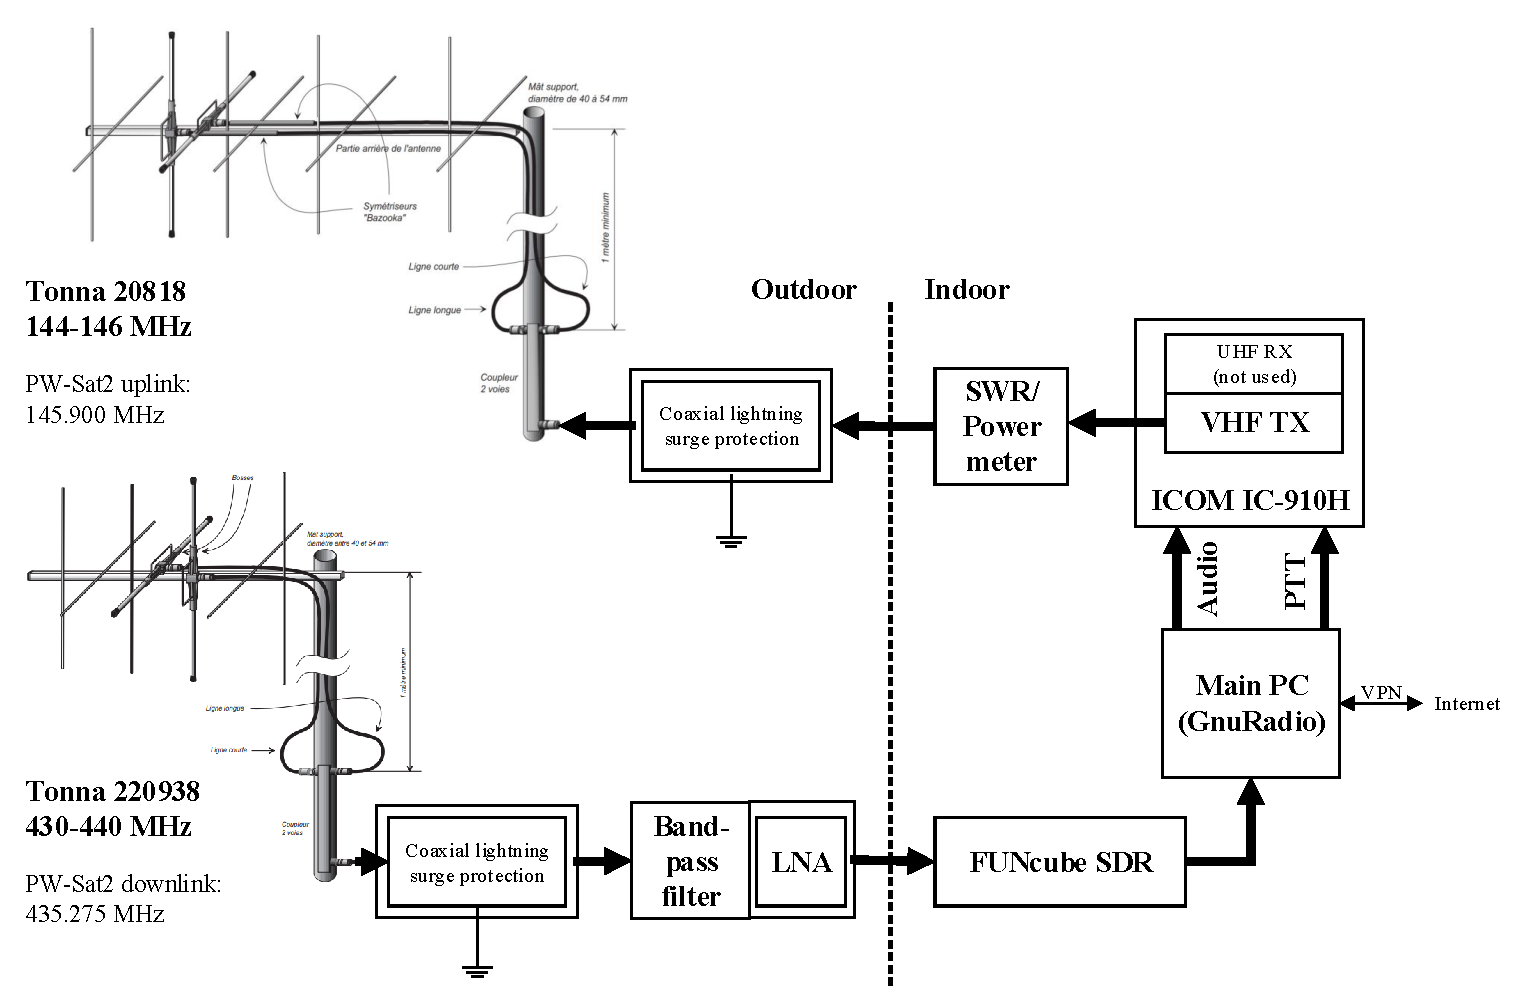
\includegraphics[width=0.8\paperwidth]{img/5/gs_block_diagram.eps}
    \caption{Ground station block diagram}
    \label{gs_block_diagram}
\end{figure}


\section{Antennas}
PW-Sat2 is transmitting radio signals with linear polarization, nevertheless ground station  polarization should be circular, due to the random tumbling of the satellite. This will reduce the gain of the antennas, but the signal strength will be constant regardless of the satellite rotation. Cross-Yagi antennas were selected, and two linear planes antennas were phased with coaxial cable and symmetrical splitters/combiners. Coaxial cables length was calculated to achieve \SI{90}{\degree} shift between two dipoles.

Antennas were selected to be the longest possible, limited by the antenna mast height. Selected antenna characteristics:

\begin{tabular}{c|c}
     \textbf{Downlink} & \textbf{Uplink} \\ \hline
     Tonna 220938 & Tonna 20818 \\
     2x 19 elements & 2x 9 elements \\
     loop dipole & linear dipole \\
     \SI{16.2}{\dBi} gain & \SI{13.2}{\dBi} gain \\
     \SI{30}{\degree} beamwidth & \SI{40}{\degree} beamwidth
\end{tabular}

Additionally, two combiners were selected for antenna phasing: Tonna 31202 for VHF and Tonna 31270 for UHF. Antennas are also protected by the Coaxial lightning surge protection, to minimise risk of damaging indoor equipment.

\subsection{Measurements}
After the assembly, antennas should be measured to make sure of the correct assembly. The simplest method is to measure the impedance of the antennas.

Each antenna consist of two dipoles (with vertical and horizontal polarization) phased with a combiner. Measurements of the dipoles and the phased antenna were performed, and the result is shown in the table \ref{TODO}.


\section{Uplink - transmitter}
Uplink signal is an FM-modulated AFSK, so standard analog audio FM transceiver can be used to generate RF signal. The frequency deviation of the de-modulator was selected to allow to use radio amateur voice transceivers. Audio signal (before FM-modulation) is generated by the software running on the PC.

During PW-Sat1 project, the Icom 910H amateur radio transceiver was used for both uplink and downlink, therefore it was proposed to use the the same radio as it do comply with all the requirements. Radio is shown in the figure \ref{Icom_910H_ref}.

\begin{figure}[H]
    \centering
    \includegraphics[width=0.6\paperwidth]{img/5/icom910h.jpg}
    \caption{Icom 910H. Source: \cite{ICOM_910H_pic}}
    \label{Icom_910H_ref}
\end{figure}

Radio VHF FM transmit characteristics:

\begin{tabular}{c|c}
    Frequency & \si{144} - \SI{148}{\MHz} \\
    Frequency stability &  \SI{\pm 3}{\ppm} \\
    Output power & \SI{100}{\watt} \\
    Audio input & analog jack \\
    Audio bandwidth & \SI{4}{\kHz} \\
\end{tabular}

\subsection{Data flow}
This radio is connected to the computer, which controls the audio to transmit and Push-To-Talk (PTT, transmission enable) signal. Uplink baseband signal (AFSK) has generated by the GNURadio framework, to be later FM-modulated and transmitted using conventional radio. Block diagram of uplink data chain is shown in the figure \ref{uplink_data_flow}

\begin{figure}[H]
    \centering
    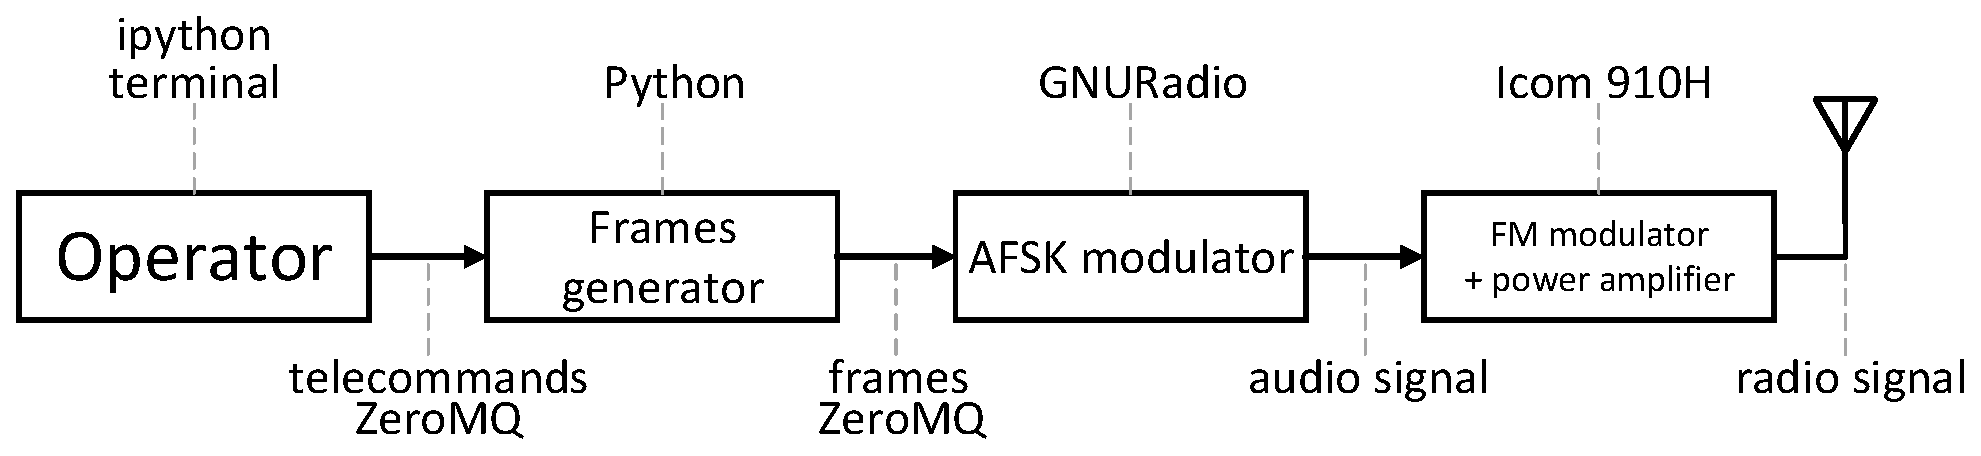
\includegraphics[width=0.6\paperwidth]{img/5/uplink_data_flow.eps}
    \caption{Uplink data flow}
    \label{uplink_data_flow}
\end{figure}

AFSK signal generation GNURadio flowgraph is shown in the figure \ref{uplink_flowgraph}. Audio signal is generated by software Voltage Controlled Oscillator (VCO), and the frequency is controlled by the actual bit value (\SI{1200}{\hertz} or \SI{2200}{\hertz}).

% TODO: uplink_flowgraph


\subsection{Standing Wave Ratio meter}
To check proper antenna connection and ensure long-term monitoring a SWR (Standing Wave Ratio) was installed. This instrument measures ratio of reflected power, thus providing information about antenna impedance matching. In case of antenna break

% TODO: zdjęcie/zrzut z kamerki SWR metera


\subsection{Measurements}
As the uplink was built using conventional HAM radio transceiver, only the modulation and output power should be measured. As the physical layer is the typical FM-modulated AFSK and frame protocol is typical AX.25 there is a lot of free software to verify the correctness of the frame and modulation.

\subsubsection{Output power}
The power of the power amplifier (built in the transceiver) was measured using an SWR \& Power Meter TODO, and by connecting radio output to the antenna. The measured output and SWR was equal to TODO. Those parameters are continuously monitored during the mission to monitor the cables and radio health.

\subsubsection{Spectrum \& Watchdogs}
The spectrum and output modulation correctness in constantly monitored using so-called watchdogs built using another Software Defined Radios (PlutoSDR, RTL-SDR) placed in the proximity of the main antennas.
By demodulating uplink signal and comparing it in the real time with transmitted frames the correctness of the transmission is guaranteed. Watchdog flowchart and graphical view are shown in the figure \ref{TODO}.



% ------------------------------------------------------------
% ------------------------- DOWNLINK -------------------------
% ------------------------------------------------------------

\section{Downlink}
Receiving Signals from maximal slant range of about \SI{3000}{\kilo\meter} from a \SI{0.5}{\watt} transmitter requires very high processing gain and low noise factor of the system. System also needs to compensate for Doppler effect and ground interferences.

\subsection{Signal front-end processing}
Radio front-end has two main purposes - to lower the system noise figure (by amplifying the signal with Low Noise Amplifier) and eliminate intermodulation with another signals (filtering). Low Noise Amplifier, installed close to the antenna reduces influence of the long cable to the receiver and reduces the noise added by receiver, reducing total system noise factor. Noise factor is limited by the attenuation between the antenna and Low Noise Amplifier and the Noise Factor of the amplifier itself. However, strong signals in the frequency proximity of the signal can intermodulate in the LNA, resulting in variety of issues: from reduced gain to completely distorted signal.

Narrow-band filter should be installed before the LNA. However, this requires the filter to have the lower loss possible, as the insertion loss of the filter directly affects noise figure of the system. For this purpose, cavity filter was selected. This, narrow band filter (\SI{1}{\MHz}), has very low insertion loss as shown in the measurement chapter. After the filter, Low Noise Amplifier is mounted.

Front-end signal processing is installed as close to the antenna as possible as shown in the figure \ref{elka_skrzynka}.

\begin{figure*}
   \centering
\begin{tabular}{cc}
        \includegraphics[width=0.3\paperwidth]{img/5/elka_view.jpg}
    & 
        \includegraphics[width=0.3\paperwidth]{img/5/elka_skrzynka.jpg}
\end{tabular}
\label{elka_skrzynka}
\caption{PW-Sat2 ground station view and front-end processing.}
\end{figure*}

\subsubsection{Filter measurements}
Cavity filter was tuned to the required frequency to minimize insertion loss and bandwidth. Signal bandwidth is very narrow compared to the filter frequency range.
The insertion loss and band pass range was measured using Network Analyser. S-parameters are shown in the figure \ref{TODO} and the filter parameters are summarised in the table \ref{TODO}.

\subsection{Low noise amplifier}
A dedicated Low Noise Amplifier was designed. It should eliminate out-of-band signals and amplify the required downlink frequency by at least \SI{20}{\dB}. As the main active component, a high-level Low Noise Amplifier: Mini-Circuits PGA-103+ \cite{lna_pga_datasheet} was used. Additional \SI{433}{\MHz} SAW filter was placed before the amplifier to reduce out of band interferences signals. Bias of the amplifier is created by RF Low Dropout Regulator Texas Instruments TPS7A47 \cite{lna_ldo_datasheet}. Amplifier was designed to support two-stage configuration, but for PW-Sat2 only first stage was populated. Schematic, PCD layout and the picture of the designed board are shown in the figures: \ref{lna_schematic} and \ref{lna_pcb}. The design is open source and all the source files can be found at \cite{lna_github}

\begin{figure}[H]
    \centering
    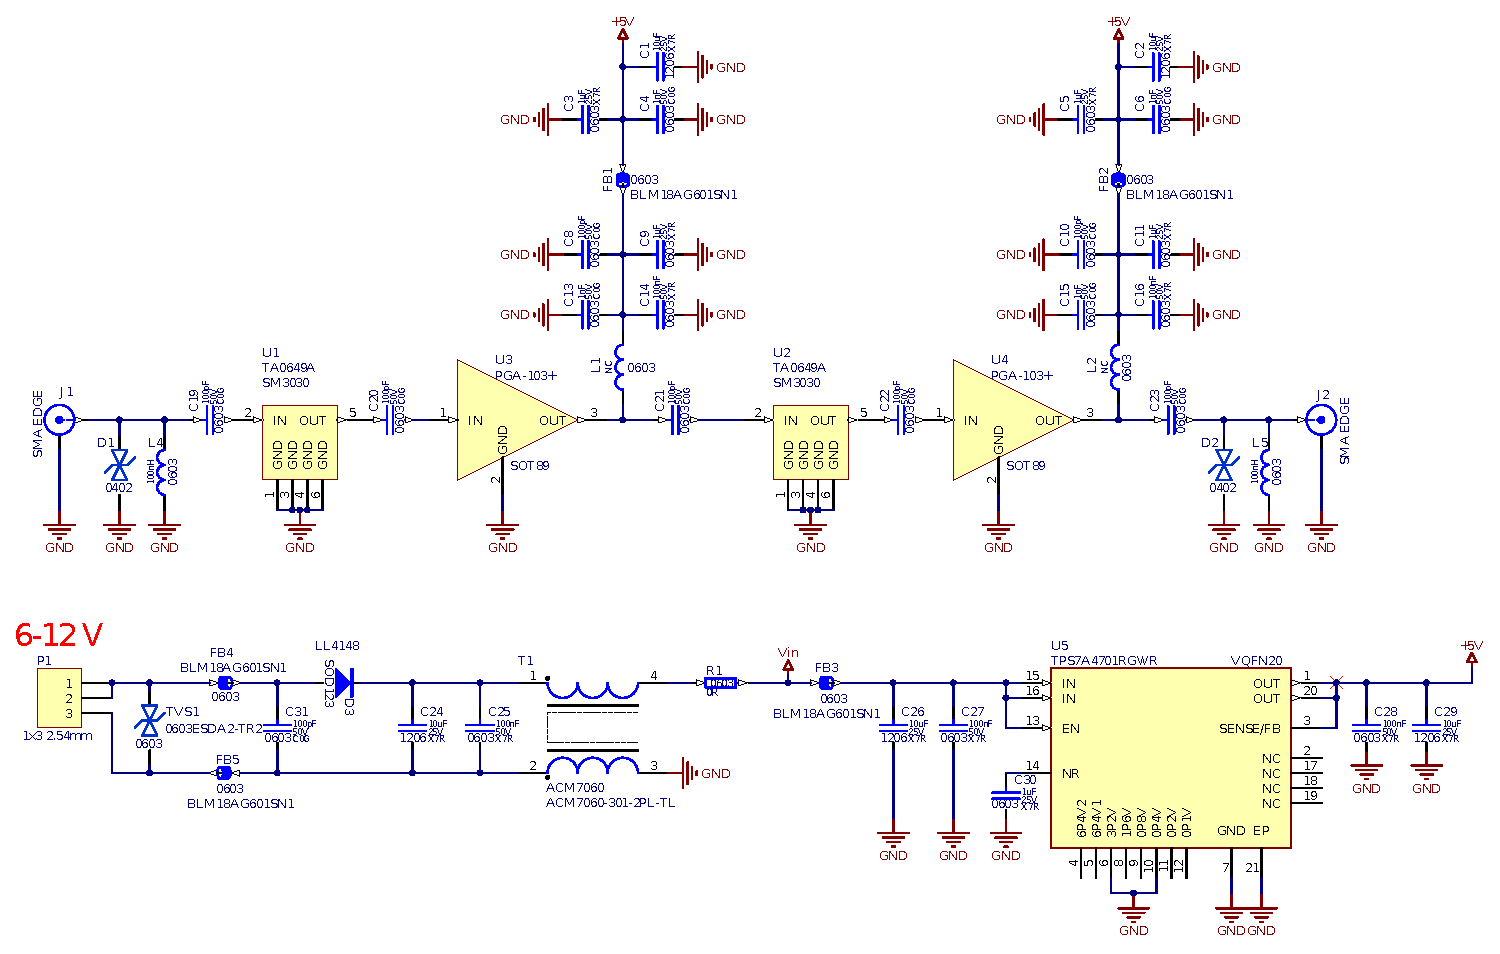
\includegraphics[width=0.8\paperwidth]{img/5/lna_schematic.eps}
    \caption{Low Noise Amplifier Schematic}
    \label{lna_schematic}
\end{figure}

\begin{figure*}
   \centering
\begin{tabular}{cc}
        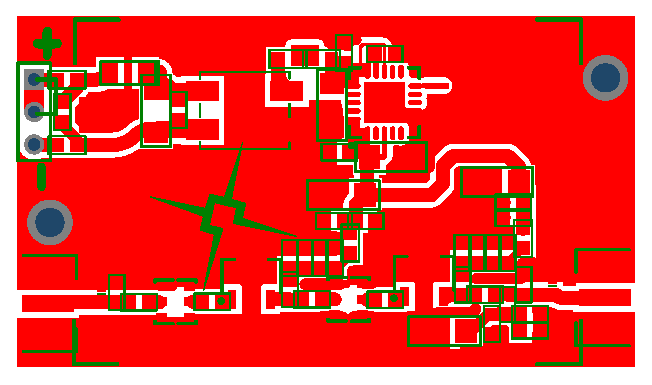
\includegraphics[width=0.4\paperwidth]{img/5/lna_pcb.eps}
    & 
        \includegraphics[width=0.3\paperwidth]{img/5/lna_assembled.jpg}
\end{tabular}
\label{lna_pcb}
\caption{Low Noise Amplifier PCB layout and assembled picture}
\end{figure*}


\subsubsection{Measurements}
Designed Low Noise Amplifier is shown in the figure \ref{TODO}. Its S-parameters were tested using Rohde\& Schwarz ZVL. Results are shown in the figure \ref{TODO}. Gain and frequency were as expected and are shown in the table \ref{TODO}.


\subsection{Receiver}
Due to the custom packet format no commercially available integrated circuits were able to correctly receive packets, therefore a custom solution was required for de-modulation and packet recovery.
To receive BPSK signals, the phase recovery is necessary. One of the methods of the synchronous detection is the use of Costas loop \cite{costas_loop}. Most simple solution is to implement full signal chain: Costas loop, bit recovery and packet formatting into software, therefore requiring down-conversion of the signal and data transfer to the PC. 

One of the possible and widely used methods is to use radio amateur transceiver in SSB mode - then radio acts as a multi-stage down-converter, allowing to receive baseband with audio card from PC. However, due to main purpose of transmitting audio signals, there is a lowpass filter for baseband at about \SI{3}{\kHz}. Using SSB mode for receiving PW-Sat2 is possible, however only for \SI{1.2}{\kbps} bitrate.

Another method was to use Software-Defined Radio, performing IQ downconversion and data transmission. The Radio Amateur Satellite Corporation designed an SDR receiver for their mission FUNcube Satellite. After mission success, they released their design and started selling FUNcube dongle shown in the figure \ref{funcube_pic}. Given that is was designed specifically for satellite communication and it was tested using similar CubeSat design, it was selected as the main receiver for PW-Sat2.

\begin{figure}[H]
    \centering
    \includegraphics[width=0.6\paperwidth]{img/2/funcube.jpg}
    \caption{FUNcube Dongle Pro+. Source: \cite{funcube}}
    \label{funcube_pic}
\end{figure}

The receiver  functionalities:
\begin{itemize}
    \item Doppler correction,
    \item IQ data recording,
    \item BPSK demodulation,
    \item bit recovery,
    \item packet formatting,
    \item multiple bitrate simultaneous decoders,
    \item sending data on-line to the operators,
    \item work with different Software-Defined Radios and SSB transceivers
\end{itemize}

The block diagram of the designed system is shown in the figure \ref{demodulator_block_diagram}. All of the signal processing blocks were created using GNUradio framework.

\begin{figure}[H]
    \centering
    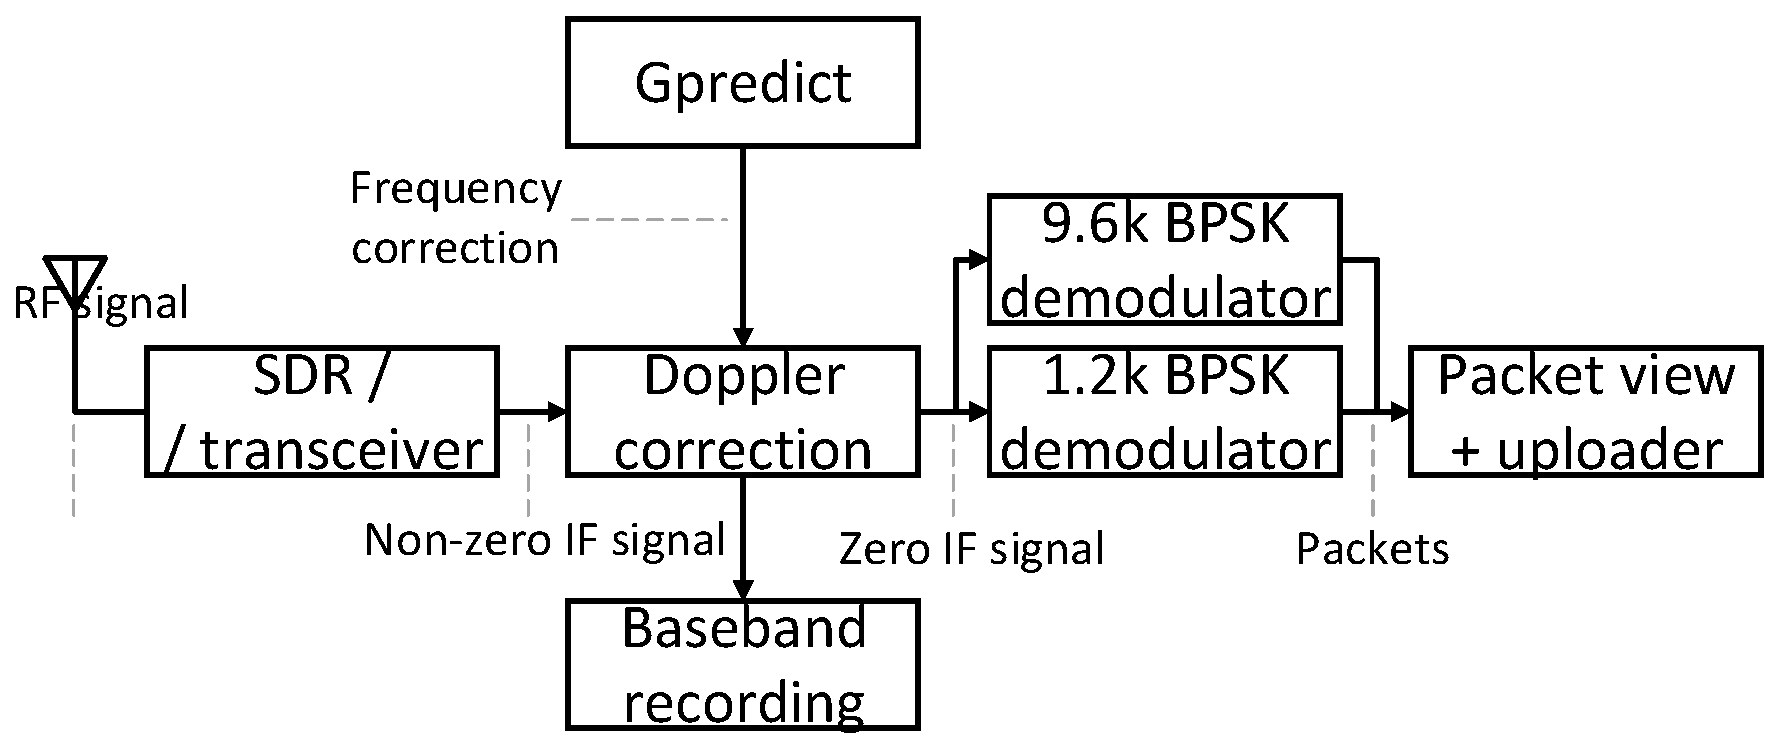
\includegraphics[width=0.6\paperwidth]{img/5/demodulator_block_diagram.eps}
    \caption{Demodulator Block Diagram}
    \label{demodulator_block_diagram}
\end{figure}

First stage, the SDR / transceiver can be any type of Software-Defined radio working with osmocom device drivers, FUNcube SDR or analog SSB radio using audio card. To mitigate the DC-offset and IQ imbalance, the output of this block is on non-zero IF - the frequency of the PW-Sat2 is shifted from the LO frequency. For SSB transceiver, it has to be tuned \SI{2}{\kHz} below the center frequency due to the limited bandwidth of the audio filters. Signal source dialog of the main application is shown in the figure \ref{gs_source_selection}.

\begin{figure}[H]
    \centering
    \includegraphics[width=0.6\paperwidth]{img/5/gs_source_selection.png}
    \caption{Ground station application - signal source selection}
    \label{gs_source_selection}
\end{figure}

Doppler correction is build on quadrature mixer and create zero-IF signal for the next processing blocks. Gpredict calculates required frequency shift and sends it to the block via TCP/IP connection. This updates local VCO frequency for the down-conversion. Latter, the signal is fist-stage filtered and saved to the file for logging purposes. GNUradio block diagram is shown in the figure \ref{gs_doppler_gnuradio}.

\begin{figure}[H]
    \centering
    \includegraphics[width=0.6\paperwidth]{img/5/gs_doppler_gnuradio.png}
    \caption{Doppler correction block GNUradio flowgraph}
    \label{gs_doppler_gnuradio}
\end{figure}

In the system, there are two demodulators (for \SI{1.2}{\kbps} and \SI{9.6}{\kbps} bitrates) operating simulateneously. This allows immediate signal reception during bitrate change by the operator without any manual intervention in the software. Each of them consists of couple of blocks, as shown in the figure \ref{gs_demodulator_diagram}. The demodulator has its own GUI  to show user the status of the demodulation, as shown in the figure \ref{gs_demodulator_gui}.
\begin{itemize}
    \item filtering - low-pass signal with matched Root Raised Cosine filter to eliminate out of band noise,
    \item Costas loop - carrier recovery and phase demodulation,
    \item Symbol synchronisation - recovers bits from the baseband signal, locking a PLL onto the signal,
    \item packet framing - builds a frame from stream of bits,
    \item frame pass to the higher level software.
\end{itemize}

\begin{figure}[H]
    \centering
    \includegraphics[width=0.6\paperwidth]{img/5/gs_demodulator_diagram.png}
    \caption{Ground station demodulator GNUradio flowgraph}
    \label{gs_demodulator_diagram}
\end{figure}

\begin{figure}[H]
    \centering
    \includegraphics[width=0.6\paperwidth]{img/5/gs_demodulator_gui.jpg}
    \caption{Ground station demodulator GUI}
    \label{gs_demodulator_gui}
\end{figure}

The demodulator was designed for two major cases:
\begin{itemize}
    \item wide bandwidth and large frequency correction (when orbit Keppler data is not well-known, resulting in unpredicted Doppler shift),
    \item wide bandwidth and no frequency correction (when orbit Keppler data is well-known resulting in negligible frequency inaccuracies).
\end{itemize}

Depending on the case, different parameters of the Costa's loop were determined. Both test-cases were implemented and the sensitivity and maximum frequency shift were determined.

After the packet reception, it is shown for the user (as in the figure \ref{gs_frame_view}) and uploaded to the cloud for further analysis by the operations team.

\begin{figure}[H]
    \centering
    \includegraphics[width=0.6\paperwidth]{img/5/gs_frame_view.png}
    \caption{Ground station received frame view}
    \label{gs_frame_view}
\end{figure}


\subsubsection{Measurements}
Frequency correction block was tested using already flying satellites, verifying stability of frequency after correction.

The test setup for measuring demodulator is shown in the figure \ref{TODO}, and consist of:
\begin{itemize}
    \item PlutoSDR - transmitter of the frames with regulated center frequency and output power,
    \item attenuators
    \item Funcube Pro+ SDR - receiver used in the ground station
\end{itemize}

Frames to be transmitted were recorded with Software-Defined Radio during flatsat campaign and replayed during sensitivity tests. This ensures that all the important inadequacies transmitted by the radio transmitter were also taken into account.
With the test setup, sensitivity was automatically measured by varying output power of the transmitter (in \SI{0.25}{\dB} steps) and PER was recorded for each point. During the process, different parameters of the demodulator were tuned to increase the sensitivity. Final results are shown in the table \ref{TODO} and figures \ref{TODO} - \ref{TODO}.
